\bookchapter{Chapter 37: The Paradigm Shift — From Writing Code to Directing AI}

\chapterintro{Congratulations — by opening this book you're standing in the middle of a professional paradigm shift. It started with one programmer's social post in 2025. Dramatic? It really happened that way.}

\booksection{The birth of Vibe Coding: A movement sparked by one sentence}

In February 2025, Andrej Karpathy — remember this name, you'll see it again — posted a tweet that got quoted over and over: “There's a new kind of coding called Vibe Coding, where you fully give in to the vibes, ignore the code details, and let AI handle everything. You say what you see, copy-paste, and basically it just works.”

That casual-sounding remark precisely named a paradigm shift already underway: humans no longer write code line by line. Instead, we describe intent in natural language and AI implements it. Karpathy's wording was playful, but the insight is deep: once AI code generation crossed a threshold, the bottleneck stopped being “can I write this line?” and became “can I think this through clearly?”

\begin{tcbinfo}{Quick tip: What's a "vibe"?}
“Vibe” means mood or feel. Vibe Coding is “directing AI coding by feel” — you describe what you want, AI implements it. Remember the term; it's this movement's birth certificate.

\end{tcbinfo}

From that moment, “coding” split in two: classic coding turns designs into syntax; new coding turns intent into instructions. The first tests your fingers; the second tests your brain.

Vibe Coding quickly moved from joke to serious engineering concept. By mid-2026 it had grown from a social-media meme into a full methodology covering requirements, context management, iterative validation, and quality assurance. People also realized “coding by vibes” is only the beginner stage — truly efficient AI coding needs a systematic way of thinking. That way of thinking is what this book gives you.

\booksection{2026 status: The Agentic Engineering era}

By August 2026, AI coding had gone through several paradigm shifts. Vibe Coding was the first spark, but people soon found that pure vibes + chat produced wildly unstable code — brilliant sometimes, broken others. So the paradigm evolved: from casual chat coding toward structured agent engineering.

Karpathy again — in early 2026 he proposed Agentic Engineering. Unlike Vibe Coding's “say it and it generates,” Agentic Engineering means: give AI a goal and let it plan steps, call tools, verify results, and iterate. AI is no longer just a code generator; it's an agent that perceives its environment, makes decisions, and takes actions.

This shift brought three key changes:

\begin{enumerate}
  \item Interaction changed: From "one question, one answer" to "set the goal, then delegate."
  \item Deliverables changed: From "a piece of code" to "a complete project."
  \item Your role changed: From "review every line" to "define boundaries and accept results."
\end{enumerate}

The numbers don't lie: In Cursor 3, released April 2026, Agent mode usage overtook Tab completion for the first time — a clear sign developers had shifted at scale. Claude Code, the terminal-native AI coding tool, hit a \$2.5 billion annualized revenue run rate by mid-2026. The chart below shows that crossover moment:

\begin{center}
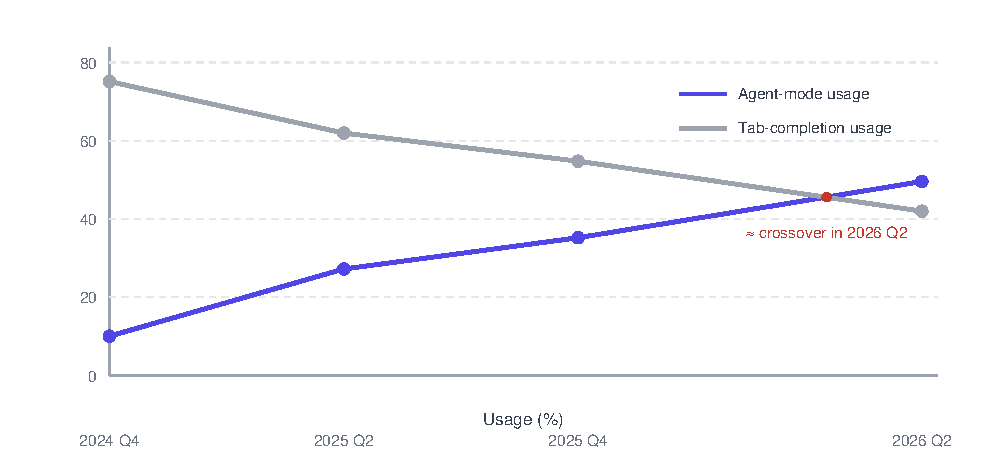
\includegraphics[width=0.92\linewidth]{figures/fig-di-san-shi-qi-zhang-1}
\\[2pt]\small Figure 1: AI coding interaction-mode usage trends (estimated from industry research; Agent mode overtakes Tab completion in 2026 Q2)
\end{center}

Honest truth: tools and models change, but successful AI coding practitioners follow the same underlying methodology whether they use Cursor or Claude Code, GPT-5 or Claude 4.5. That methodology is what this guide teaches.

\booksection{The core mindset shift: From Coder to Conductor}

Traditional coding education teaches you to be a Coder — understand syntax, memorize APIs, debug logic. In the AI coding era, that role is being redefined. You no longer need to type every line yourself. Instead, become a Conductor: define the battlefield, set rules, assign tasks, accept results.

The shift isn't about “can you write code” — it's about “can you think clearly about what to build.” A great conductor isn't necessarily the best soldier, but they know the objective, terrain, and troop placement best. Likewise, a great AI coding practitioner doesn't need every syntax detail memorized, but must be crystal clear on goals, architectural constraints, and quality standards.

Worth reading twice — this table captures the whole role change:

\begin{center}
\begin{tabularx}{\linewidth}{|X|X|X|}
\hline
\textbf{Dimension} & \textbf{Traditional Coder} & \textbf{AI Conductor} \tabularnewline
\hline
Core skills & Syntax memory, API calls, debugging & Requirements definition, context management, acceptance judgment \tabularnewline
How you work & Write code line by line & Describe intent, review output \tabularnewline
Quality control & You know it because you wrote it & Verify AI output with tests and review \tabularnewline
Knowledge needed & Deep mastery of a language/framework & Broad tech literacy, deep business logic understanding \tabularnewline
Where the bottleneck is & Typing speed and syntax memory & Clarity of thought and communication \tabularnewline
Where errors come from & Syntax bugs, logic gaps & Vague requirements, missing context \tabularnewline
\hline
\end{tabularx}
\end{center}

\begin{center}\small\color{gray}Traditional Coder vs. AI Conductor — capability comparison\end{center}

This does NOT mean coding knowledge is obsolete. Far from it: you can only review and correct AI code if you can read it; you can only judge whether AI's design is sound if you understand data structures and algorithms. Knowledge sets your “conductor ceiling” — but its role shifts from “execution tool” to “judgment basis.”

\booksection{Why methodology beats tools}

Tools iterate every three months; methodology evolves only every three years. Learn a tool's mechanics and it may be obsolete in three months; master a way of thinking and it still applies three years later.

Many beginners ask first: “Which tool is best?” “Which model is strongest?” Those questions aren't unimportant — they're just the wrong priority. The 2026 tool landscape looks nothing like 2025: Trae and Qoder rose and fell, Cursor went from plugin to standalone IDE to Cursor 3, Claude Code went from experiment to terminal-coding mainstream. Yet behind all that churn, the thinking principles of successful practitioners barely changed.

That's why this book won't waste pages on one tool's button-by-button walkthrough — those go stale the moment they're written. Instead, it focuses entirely on a proven thinking methodology: how to think about requirements, how to talk to AI, how to verify output, how to keep iterating. Master this and any tool is quick to pick up. Learn only tool steps and every new tool starts you from zero.

\begin{tcbinfo}{Reassurance for absolute beginners}
If you're starting from zero, don't let “methodology” scare you. It's not abstract philosophy — it's an operator's manual for “how to think when something breaks.” Like cooking: you can follow a recipe (tool steps), but a real chef understands “why season this way” and “how to control heat” (methodology). This book starts from the basics, pairs every principle with concrete examples, and makes sure you understand both “what” and “how.”

\end{tcbinfo}

\begin{tcbpractice}{Hands-on: Take a "role photo" of yourself today}
On a piece of paper, answer three questions: (1) How do you currently use AI to write code (if at all)? (2) Are you more like the “Coder” or the “Conductor” in the table above? (3) How would you like to describe your workflow three months from now? Tuck it in the book and revisit after Chapter 47 — you'll be surprised how fast things change.

\end{tcbpractice}

\begin{tcbsummary}{Chapter recap}
\begin{itemize}
  \item In 2025 Karpathy named the AI coding revolution "Vibe Coding": from line-by-line coding to describing intent in natural language
  \item By 2026 it evolved into Agentic Engineering: set goals, delegate, AI plans and executes, humans accept results
  \item Cursor 3's Agent mode overtook Tab completion; Claude Code hit \$2.5B annualized revenue
  \item Your new role is Conductor: define the battlefield, set rules, assign tasks, accept results
  \item Tools iterate every three months; methodology every three years — learn methodology, not buttons
\end{itemize}

\end{tcbsummary}
